\documentclass{beamer}
\usepackage{amsthm}
\usepackage{amsmath}
\usepackage{amsfonts}
\usepackage{amssymb}
\usepackage{epic}
\usepackage{graphicx}
\usepackage{epstopdf}
\usepackage{multirow}
\usetheme{Berlin}
\usecolortheme{seahorse}
\usepackage{multicol}



\newtheorem{question}{Question}[section] 

\title{Project 1: American Community Survey}


\author{Andrew Bernath, Heather Kitada, Ethan Edwards, Nandhita Narendra Babu}


\institute{Oregon State University}
\date

\begin{document}

\begin{frame}
\titlepage
\end{frame}

\begin{frame}{\contentsname}
\begin{multicols}{2}
\tableofcontents
\end{multicols}
\end{frame}

\section{Overview and Questions of Interest}
\begin{frame}
\frametitle{Introduction }
\begin{itemize}
\item Statistics draws together diverse backgrounds
\item Some projects require several different summaries from a single dataset
\begin{itemize}
\item ACS is a large \emph{sandbox} to play in
\end{itemize}
\item Given four group members it is natural that there would be four different areas of interest
\end{itemize}

\end{frame}

\subsection{Questions of Interest}
\begin{frame}
\frametitle{Questions of Interest }
\begin{enumerate}
\item Is there a difference in travel time between Portland and Los Angeles? 
\begin{itemize}
\item Applications in urban sprawl, traffic circulation, etc...
\end{itemize}
\item Is there a spatial relationship in predominant energy type usage accross states?  Is there a relationship between median bill cost for various energy types?
\begin{itemize}
\item Applications in solar energy (sustainable energy alternatives)
\end{itemize}
\item How do proportions of self-sufficient veterans differ from state to state?
\begin{itemize}
\item Applications in veteran health care 
\end{itemize}
\end{enumerate}
\end{frame}

\section{Findings}
\begin{frame}
\frametitle{Findings}
Topics 
\begin{enumerate}
\item Transportation Type 
\item Energy Type 
\item Veteran Disability and Benefits
\item Immigration 
\end{enumerate}

\end{frame}

\subsection{Transportation Type}
\begin{frame}
\frametitle{Transportation Type}
\begin{center} 
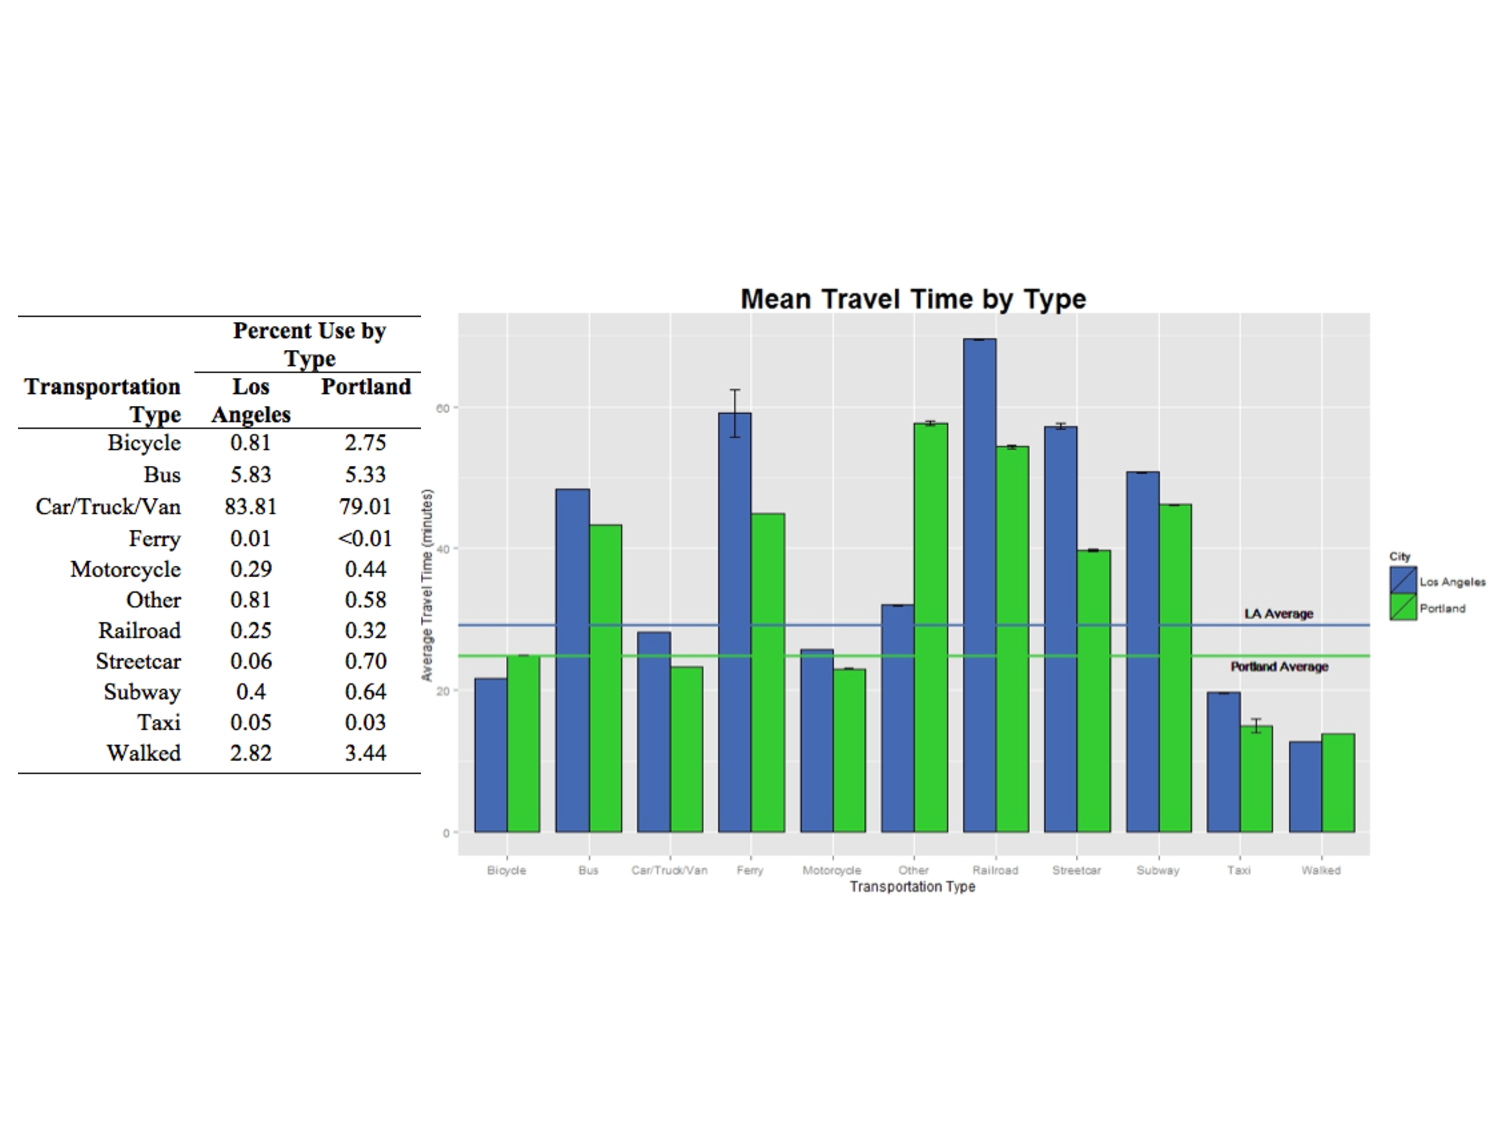
\includegraphics[width=1 \textwidth]{AndrewPlot}

\end{center}


\end{frame}


\begin{frame}
\frametitle{Transportation Type:Take Home Message}
\begin{itemize}
\item Motor vehicles still the most predominant form for commuting
\item Cycling and walking = longer commutes in Portland?
\begin{itemize}
\item Higher proportions using these forms
\item Indicative of sprawl - Los Angelians won't walk/cycle unless they are close
\end{itemize}
\item Longer commute times are not necessarily bad!
\begin{itemize}
\item Higher proportion of use = more contribution to mean
\item Interesting discovery - Portlanders love their sustainable forms!
\item Walking, Cycling, Subway
\end{itemize}
\item Perhaps most interesting: only one person commutes by ferry in Portland!
\end{itemize}

\end{frame}


\subsection{Energy Type}
\begin{frame}
\frametitle{Energy Type}
\begin{center} 
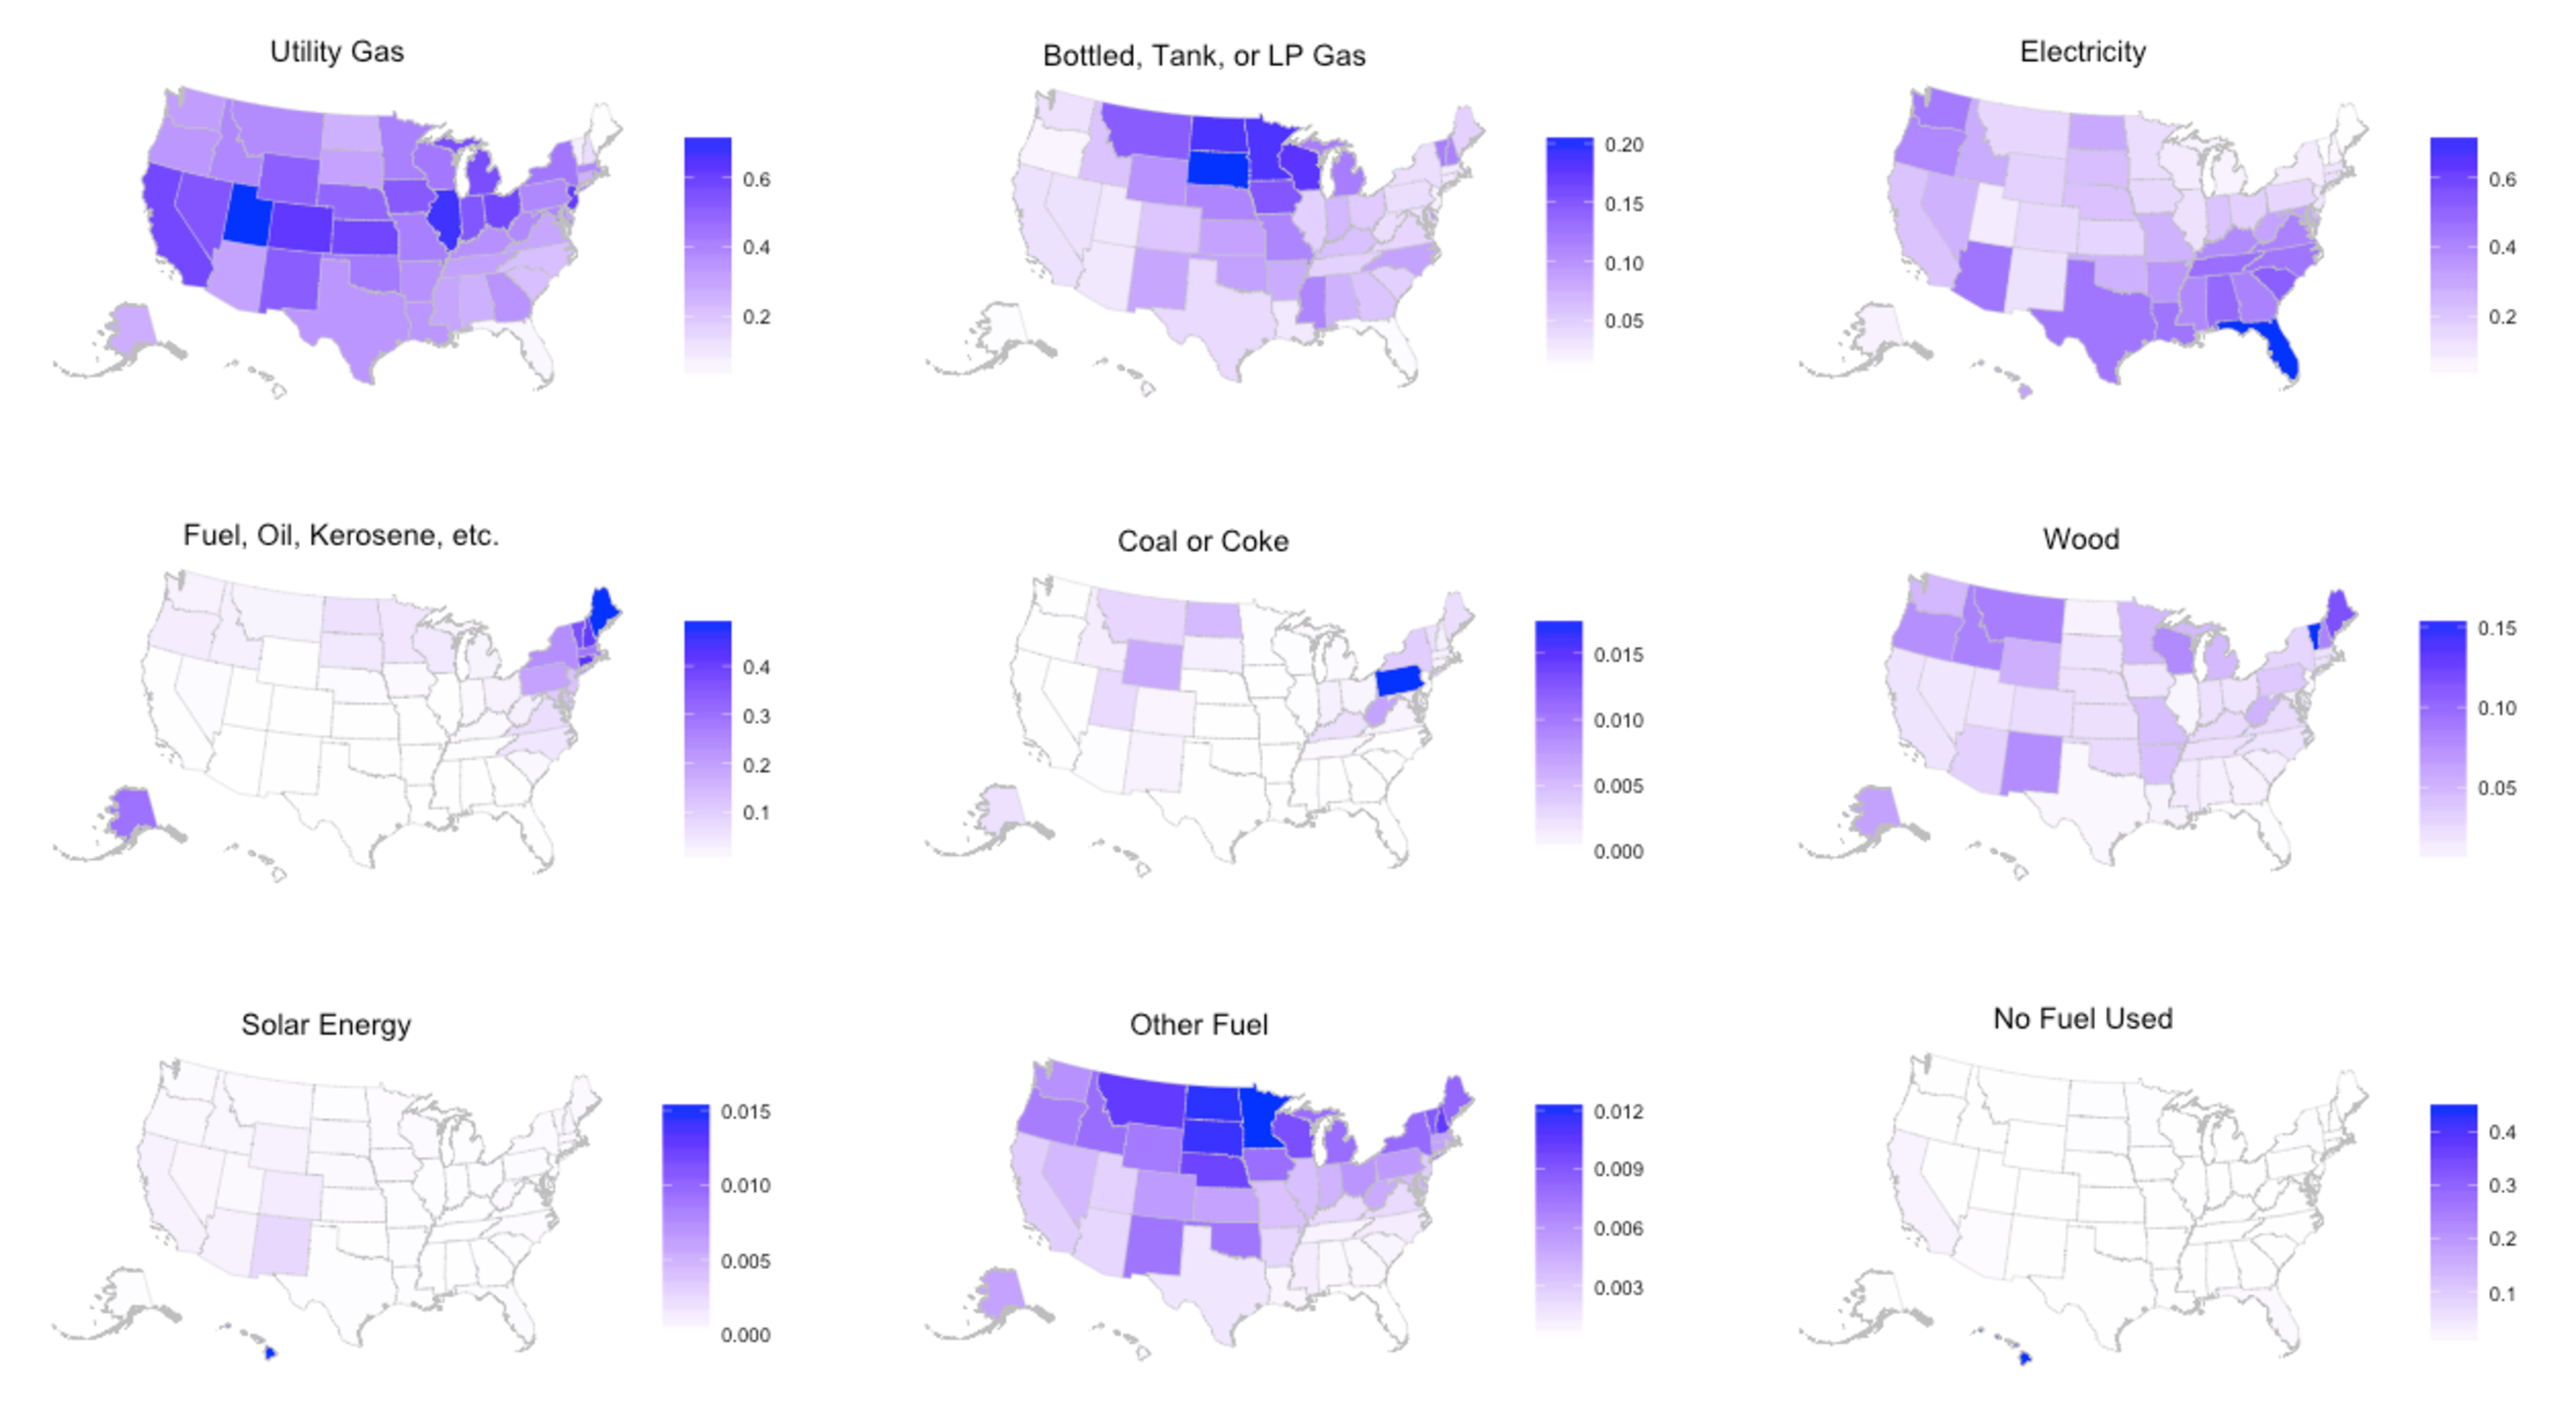
\includegraphics[width=1 \textwidth]{AllStatesEnergyTypes}

\end{center}


\end{frame}


\begin{frame}
\frametitle{Energy Type}
\begin{center} 
\includegraphics[width=.9 \textwidth]{Bills}

\end{center}


\end{frame}

\begin{frame}
\frametitle{Energy Type:Take Home Message}


\end{frame}

\subsection{Veteran Disability and Benefits}
\begin{frame}
\frametitle{Veteran Disability and Benefits}
%\begin{center} 
%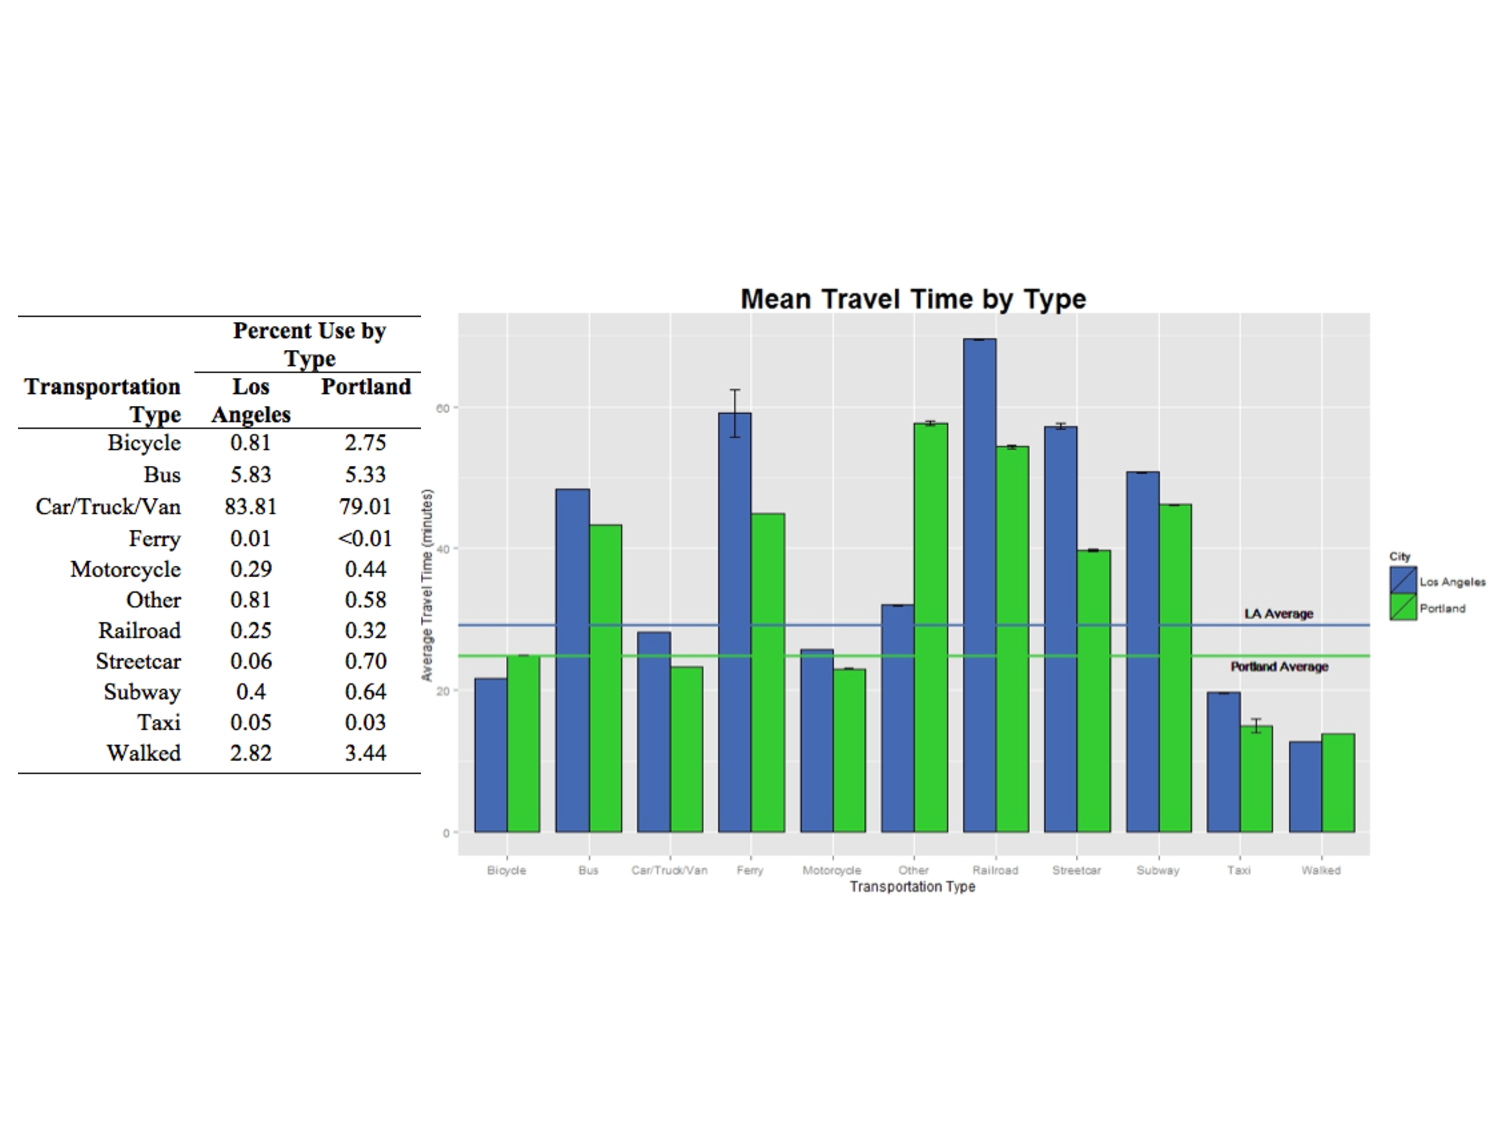
\includegraphics[width=1 \textwidth]{AndrewPlot}

%\end{center}


\end{frame}

\begin{frame}
\frametitle{Veteran Disability and Benefits:Take Home Message}
\begin{itemize}
\item Observed spatial patterns with some outliers
\begin{itemize}
\item Highest incidence rate in the Deep South
\item Lowest incidence rate in the northernmost South
\item Texas doesn't follow the Deep South pattern - the problem may not be in enlistment rates/political leaning!
\end{itemize}
\item Minor shifts in disability rating
\begin{itemize}
\item MS: Higher incidence of 10\%, 50\%-100\%, and electing out
\item ND: Higher incidence of 20\%-40\%
\end{itemize}
\end{itemize}

\end{frame}

\subsection{Immigration }
\begin{frame}
\frametitle{Immigration }
%\begin{center} 
%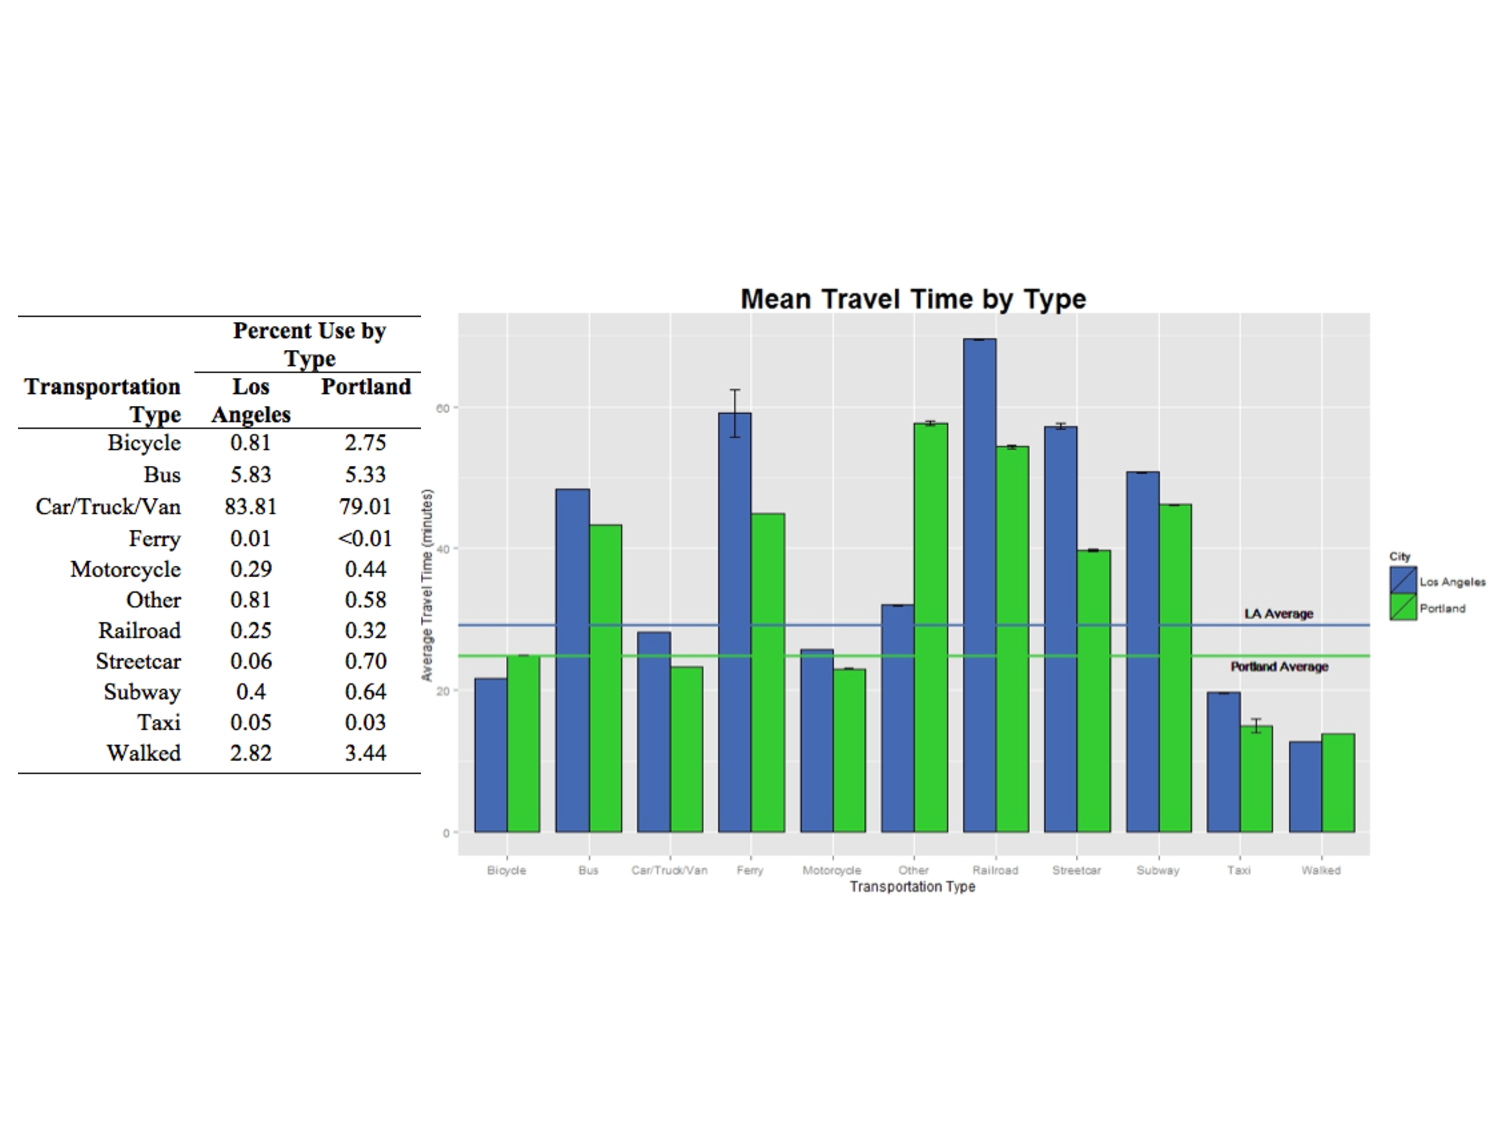
\includegraphics[width=1 \textwidth]{AndrewPlot}

%\end{center}


\end{frame}


\begin{frame}
\frametitle{Immigration :Take Home Message}


\end{frame}



\section{Obstacles and Solutions }
\begin{frame}
\frametitle{Obstacles and Solutions}
Universal:
\begin{itemize}
\item NA's in dataset
\item Communication: Online tools (Google Groups and Google Drive)
\item Continuity of project
\item General github problems
\end{itemize}
\end{frame}

\begin{frame}
\frametitle{Obstacles and Solutions}
Individual:
\begin{itemize}
\item Transportation: Coding of light rail and determining scope of areas to compare
\item Energy: Coding of data
\item Veterans: "NA" vs "Elected Not To Answer"
\item Immigrants: Technology and graphical display
\end{itemize}
\end{frame}

\section{Future Questions and Work}
\begin{frame}
\frametitle{Future Questions}
\begin{itemize}
\item Incorporate sample weights and post-stratification 
\item Assess missing information 
\item Public policy applications 
\end{itemize}
\end{frame}




\end{document}
?